U některých her je potřeba, aby měl hráč zařízení, které bude moci nosit s sebou a které mu při hře bude sloužit jako identifikace nebo nástroj pro plnění úkolů.
Takové zařízení by mělo být co nejmenší a co nejlehčí, aby hráče při hře nezdržovalo.
Navíc by mělo být co nejlevnější, aby tolik nevadilo, když jej některý hráč třeba ztratí, což se přeci jen může stát.
Mimo to toto zařízení musí být schopno zobrazit svůj stav a převzít od uživatele jednoduchý pokyn.

% Rozhodli jsme, že toto zařízení bude svůj stav zobrazovat pomocí pěti inteligentních RGB LED a jako vstup mu budou sloužit dvě tlačítka.
% Abychom nemuseli řešit napájení, má toto zařízení USB konektor a je určeno k napájení powerbankou.
% Toto zařízení jsme nazvali SemiSemafor a jeho vzhled je na obrázku \ref{fig:SemiSemafor}.

% \begin{figure}[h]
%     \centering
%     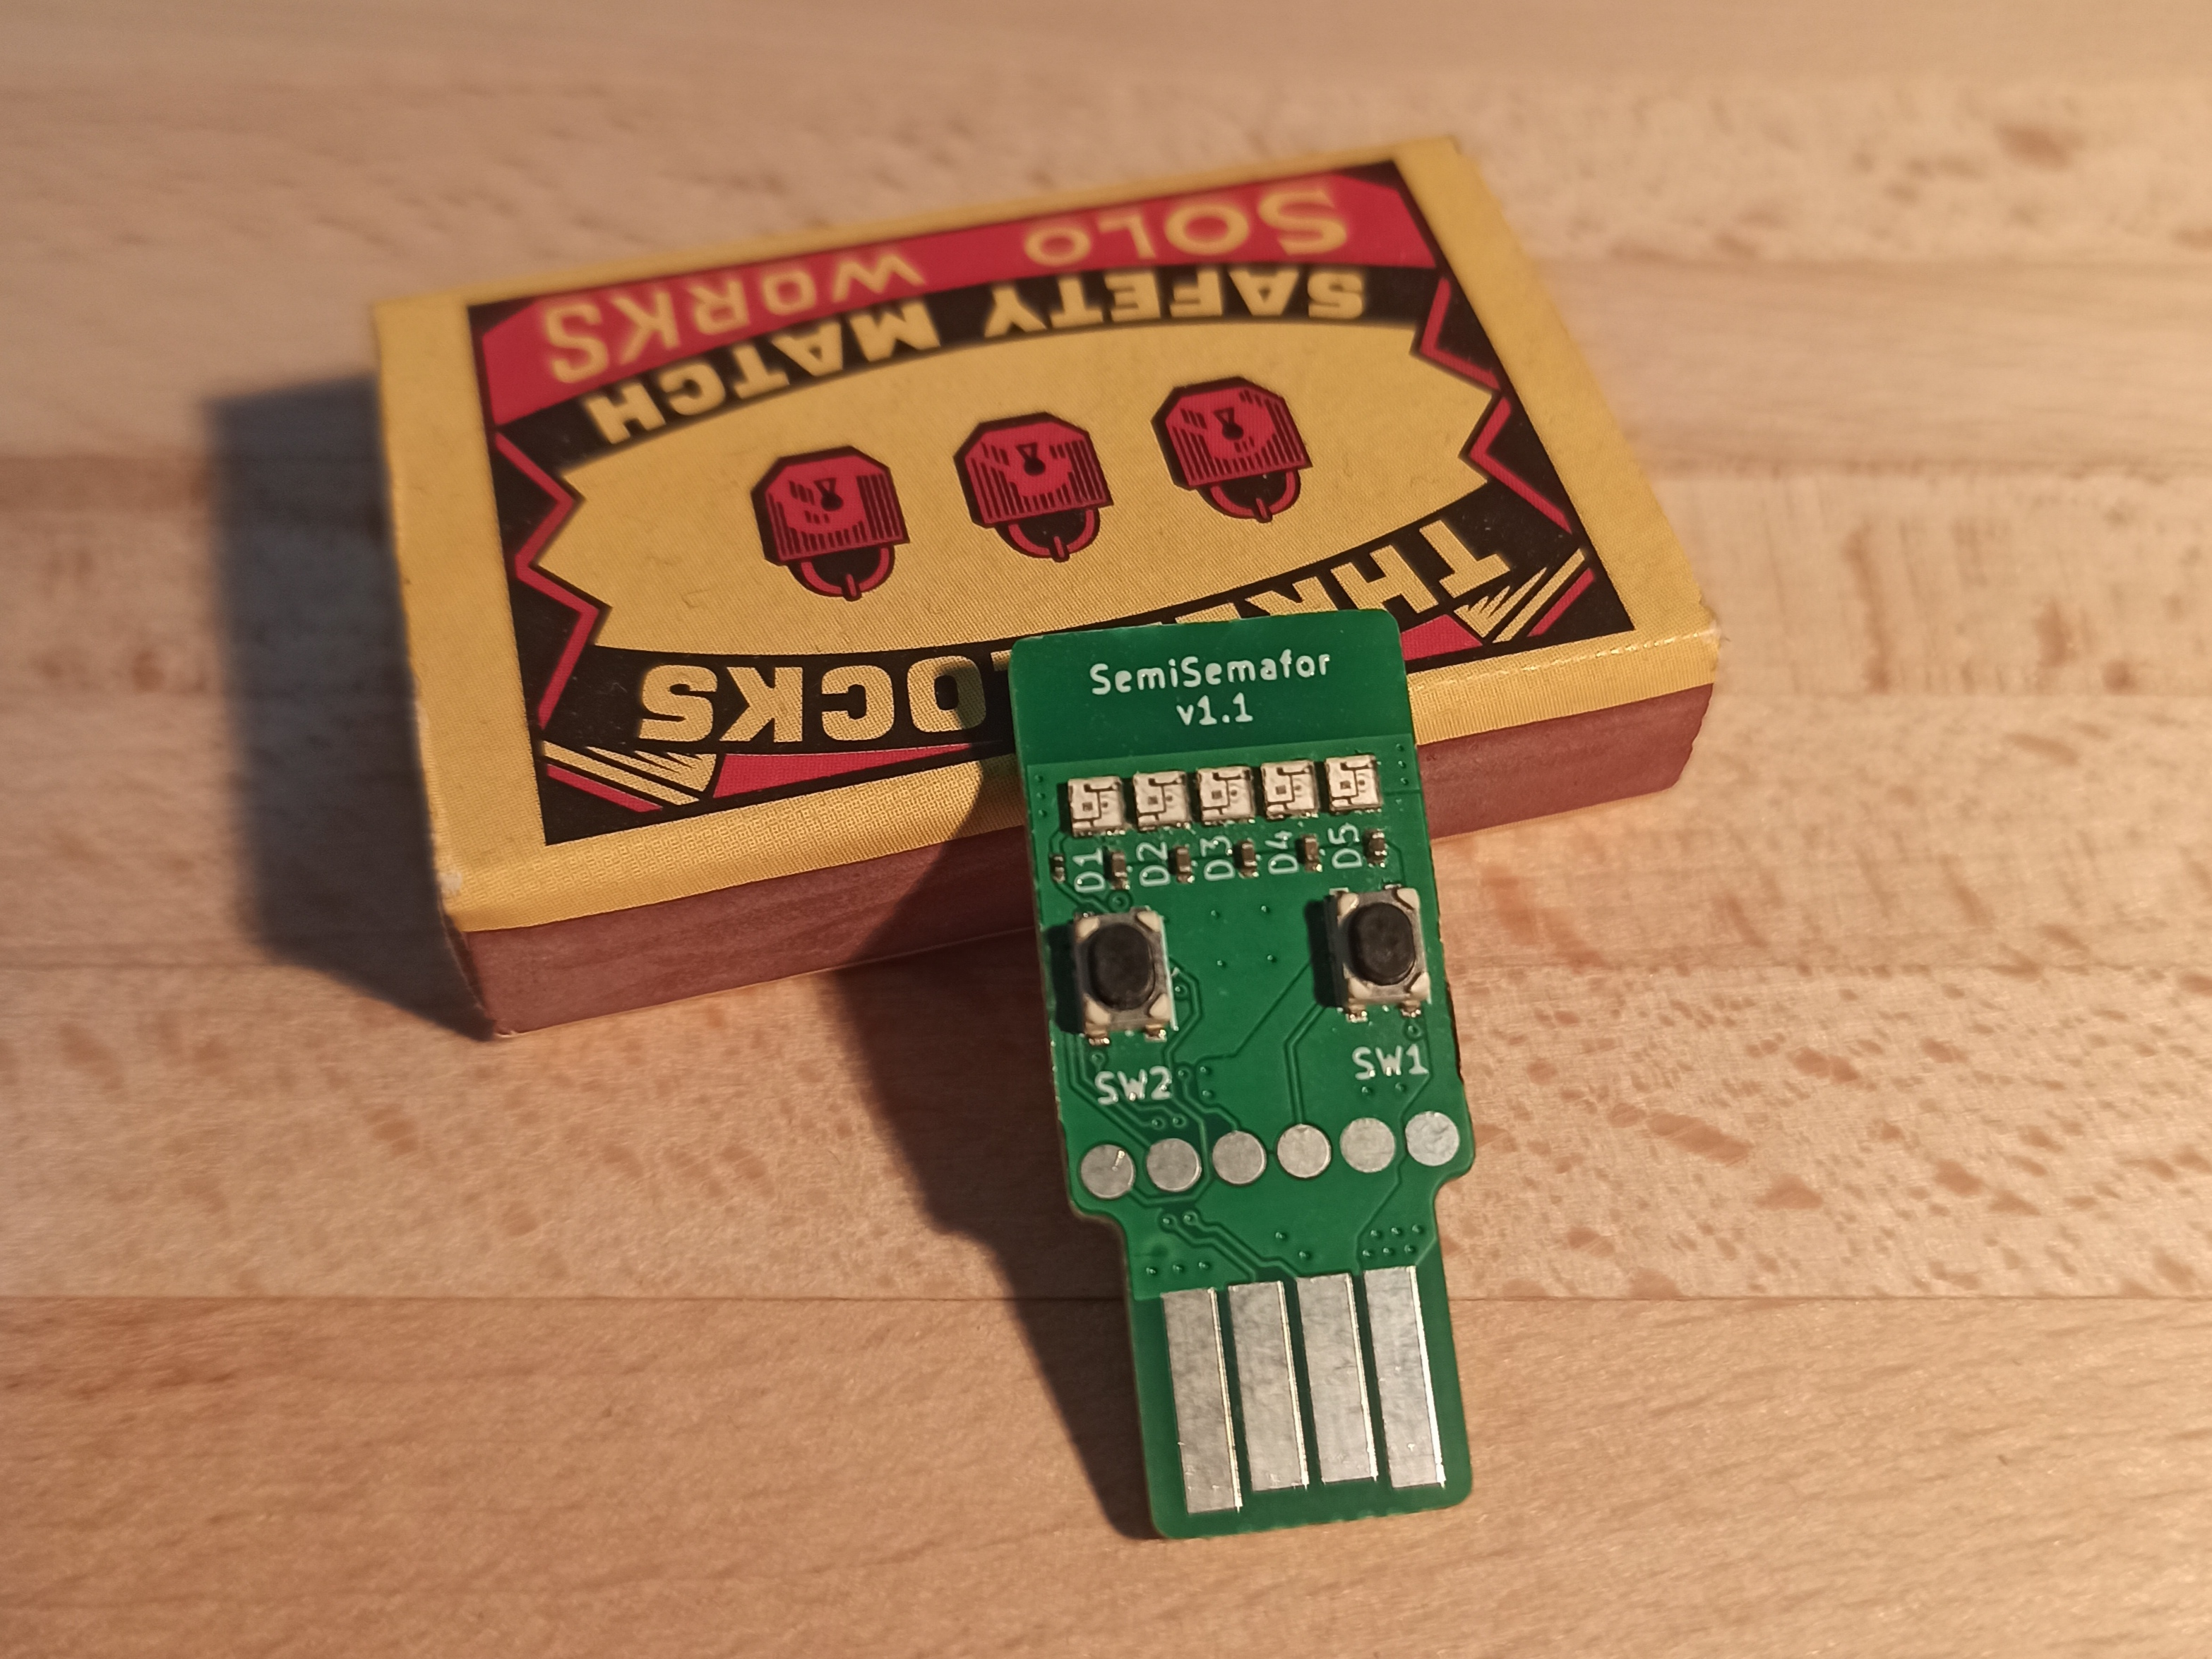
\includegraphics[width=0.8\textwidth]{text/TeoretickyUvod/AplikaceHernichZarizeni/img/1702085190411.jpg}
%     \caption{Zařízení SemiSemafor}
%     \label{fig:SemiSemafor}
% \end{figure}

% \subsection{Využití zařízení SemiSemafor}
% SemiSemafor je využitelný například ve hře s názvem Duchové.
% Nabiječa, artefakt, SemiSemafor = učastnická lucernička
% učastník dojde k nabiječce, nabije ce a u artefaktu předali energii
% lucerničky se samovibijí,
% když zmáčkneč tlačítko mužeš nabijet artefakt ale když uněj nejseš a lucernička se vybije dvakrát rychleji a odpuzuje duchy (svítí u toho bíle)
% duchová mají taky zařízení (Semiho) když drží tlačítko vybijí lucerničku i artefakty v okolí (nesvítí u toho)
% víc lidí muže naráz nabijet
% když duch chytí hráče, hráč si musí na pět minut ze hry, u nabíječky je respoun
% cílem je nabít všech tt artefaktů

% potenciálně by duchové mohli ke své činnosti potřebovat energiiž